\documentclass[10pt,a4paper]{article}

\usepackage[a4paper,top=18mm,bottom=19mm,left=18mm,right=18mm,headsep=7mm,footskip=9mm]{geometry}
\usepackage{fontspec}
\setsansfont{TeX Gyre Heros}
\setmainfont{TeX Gyre Heros}
\renewcommand{\familydefault}{\sfdefault}
\usepackage{microtype}
\usepackage{xcolor}
\usepackage{graphicx}
\usepackage{booktabs}
\usepackage{array}
\usepackage{tabularx}
\usepackage{tikz}
\usetikzlibrary{arrows.meta,positioning,calc,shapes.geometric}
\usepackage{hyperref}
\usepackage{fancyhdr}
\usepackage{caption}
\usepackage{float}
\usepackage{ragged2e}

\definecolor{Navy}{HTML}{0B132B}
\definecolor{Ink}{HTML}{172033}
\definecolor{Muted}{HTML}{667085}
\definecolor{Line}{HTML}{DDE3EC}
\definecolor{Soft}{HTML}{F5F7FB}
\definecolor{Cyan}{HTML}{00A6C8}
\definecolor{CyanSoft}{HTML}{EAF9FC}
\definecolor{Violet}{HTML}{7C5CFC}
\definecolor{VioletSoft}{HTML}{F1EEFF}
\definecolor{Green}{HTML}{12A676}
\definecolor{GreenSoft}{HTML}{EAF8F3}
\definecolor{Amber}{HTML}{F29D38}
\definecolor{AmberSoft}{HTML}{FFF5E8}
\definecolor{Rose}{HTML}{E2556F}
\definecolor{RoseSoft}{HTML}{FFF0F3}

\hypersetup{colorlinks=true,linkcolor=Cyan,urlcolor=Cyan,citecolor=Cyan,pdfauthor={HelioSat},pdftitle={Validation of the geomagnetic storm forecast}}
\setlength{\parindent}{0pt}
\setlength{\parskip}{5pt}
\setlength{\headheight}{19pt}
\setlength{\emergencystretch}{2em}
\renewcommand{\arraystretch}{1.22}
\let\plainsection\section
\renewcommand{\section}[1]{\plainsection{\color{Navy}#1}}
\let\plainsubsection\subsection
\renewcommand{\subsection}[1]{\plainsubsection{\color{Ink}#1}}

\pagestyle{fancy}
\fancyhf{}
\fancyhead[L]{\footnotesize\color{Muted}\textbf{HELIOSAT} / Geomagnetic validation}
\fancyhead[R]{\footnotesize\color{Muted}Plain-language report / August 2026}
\fancyfoot[L]{\scriptsize\color{Muted}Retrospective candidate. This is not yet an operational SLA.}
\fancyfoot[R]{\scriptsize\color{Muted}\thepage}
\renewcommand{\headrulewidth}{0.4pt}
\renewcommand{\headrule}{\hbox to\headwidth{\color{Line}\leaders\hrule height \headrulewidth\hfill}}

\newsavebox{\summarysave}
\newsavebox{\warningsave}
\newsavebox{\resultsave}
\newenvironment{summarybox}{\begin{center}\setlength{\fboxsep}{4mm}\begin{lrbox}{\summarysave}\begin{minipage}{0.90\textwidth}}{\end{minipage}\end{lrbox}\colorbox{CyanSoft}{\usebox{\summarysave}}\end{center}}
\newenvironment{warningbox}{\begin{center}\setlength{\fboxsep}{4mm}\begin{lrbox}{\warningsave}\begin{minipage}{0.90\textwidth}}{\end{minipage}\end{lrbox}\colorbox{AmberSoft}{\usebox{\warningsave}}\end{center}}
\newenvironment{resultbox}{\begin{center}\setlength{\fboxsep}{3mm}\begin{lrbox}{\resultsave}\begin{minipage}{0.91\textwidth}}{\end{minipage}\end{lrbox}\fcolorbox{Line}{white}{\usebox{\resultsave}}\end{center}}
\newcommand{\metric}[3]{\begin{minipage}[t]{0.30\linewidth}\centering{\scriptsize\color{Muted}\MakeUppercase{#1}}\\[2pt]{\fontsize{20}{22}\selectfont\bfseries\color{#3}#2}\end{minipage}}
\newcommand{\source}[1]{\textsuperscript{\color{Cyan}\textbf{[#1]}}}
\pdfstringdefDisableCommands{\def\color#1{}}

\begin{document}

\hypersetup{pageanchor=false}
\begin{titlepage}
\begin{tikzpicture}[remember picture,overlay]
  \fill[Navy] (current page.south west) rectangle (current page.north east);
  \fill[Cyan] (current page.north west) rectangle ([xshift=8mm]current page.south west);
  \fill[Cyan,opacity=0.13] ([xshift=-15mm,yshift=-24mm]current page.north east) circle (44mm);
  \fill[Violet,opacity=0.15] ([xshift=-5mm,yshift=18mm]current page.south east) circle (58mm);
  \draw[Cyan,opacity=0.28,line width=0.5pt] ([xshift=-92mm,yshift=-37mm]current page.north east) circle (27mm);
  \draw[Cyan,opacity=0.18,line width=0.5pt] ([xshift=-92mm,yshift=-37mm]current page.north east) circle (37mm);
\end{tikzpicture}
\color{white}
\vspace*{12mm}
{\small\bfseries\color{Cyan}HELIOSAT / VALIDATION \& STUDIES}\par
\vspace{32mm}
{\fontsize{30}{34}\selectfont\bfseries Geomagnetic storm\\forecasting}\par
\vspace{7mm}
{\Large\color{white!78}How we measure it, what the model learns,\\and what the results really mean}\par
\vspace{14mm}
\colorbox{Navy!75!white}{\parbox{0.72\textwidth}{\color{white}\small\vspace{2mm}A technical report written to be understood without prior knowledge of space physics or machine learning. It focuses on the practical questions: what data go in, how much warning the system provides, and how many storms it detects, misses, or alerts in error.\vspace{2mm}}}
\vfill
\begin{tabular}{@{}ll@{}}
\color{white!55}\small Data period & \color{white}\small 1995 - April 2026\\
\color{white!55}\small Final test & \color{white}\small 2024 - April 2026\\
\color{white!55}\small Customer focus & \color{white}\small G3 storms and above\\
\color{white!55}\small Status & \color{white}\small Retrospective candidate / not yet live\\
\end{tabular}
\vspace{11mm}
{\footnotesize\color{white!50}Version 1.0 / August 2026}
\end{titlepage}
\hypersetup{pageanchor=true}
\pagenumbering{arabic}

\section{The story in one minute}

The model observes the solar wind before it reaches Earth. From its speed, density, and magnetic field, it estimates the strength of the geomagnetic response. That response is expressed as Kp and, for customers, as a G1, G2, G3, G4, or G5 level.

The idea is simple: if we measure a hazardous structure upstream, near the L1 point, we can issue a warning while it travels towards Earth. In the final test, the calculated transit time has a median of \textbf{51 minutes}. This is the lead time of the observed solar-wind parcel, not a promise of the exact minute when Kp will begin to rise.

\begin{summarybox}
\textbf{Main result.} On data never used for training, from January 2024 to April 2026, HelioSat identified \textbf{16 of 27 G3+ episodes}. It issued four false G3+ alarms and missed eleven storms. Precision was \textbf{80.0\%} and recall was \textbf{59.3\%}.
\end{summarybox}

\vspace{3mm}
\begin{resultbox}
\centering
\metric{G3+ precision}{80.0\%}{Green}\hfill
\metric{G3+ recall}{59.3\%}{Cyan}\hfill
\metric{Mean Kp error}{0.44}{Violet}
\end{resultbox}

These figures are clearly better than those of the previous heuristic, but they do not yet justify a commercial SLA. The reason is statistical: 27 severe storms are still a small sample and produce wide confidence intervals. The result should be read as \textbf{promising evidence for a shadow-mode deployment}, not as an operational guarantee.

\section{What is observed, where, and from which source}

No single mission covers the whole journey. Each stage uses a different source with a specific role.

\begin{center}
\begin{tikzpicture}[node distance=8mm and 7mm,>=Latex]
\tikzset{flowbox/.style={rounded corners=2mm,minimum width=37mm,minimum height=24mm,align=center,draw=Line,fill=white,text=Ink,font=\small}, arrow/.style={->,thick,Cyan}}
\node[flowbox,fill=CyanSoft] (l1) {\textbf{1. Solar wind}\\[-1pt]\scriptsize Wind, ACE, IMP 8, Geotail\\\scriptsize through NASA OMNI};
\node[flowbox,right=of l1,fill=VioletSoft] (prop) {\textbf{2. Propagation}\\[-1pt]\scriptsize HelioSat constant-speed model\\\scriptsize from L1 to Earth};
\node[flowbox,right=of prop,fill=GreenSoft] (kp) {\textbf{3. Actual response}\\[-1pt]\scriptsize 13 ground observatories\\\scriptsize GFZ definitive Kp};
\node[flowbox,right=of kp,fill=AmberSoft] (score) {\textbf{4. Evaluation}\\[-1pt]\scriptsize alerts, hits, errors,\\\scriptsize and warning time};
\draw[arrow] (l1) -- (prop);
\draw[arrow] (prop) -- (kp);
\draw[arrow] (kp) -- (score);
\end{tikzpicture}
\end{center}

\subsection{Stage 1: upstream measurements}

The input comes from \textbf{High Resolution OMNI}, a NASA/SPDF harmonised product with five-minute resolution. OMNI is not a mission: it interleaves measurements from \textbf{Wind, ACE, IMP 8, and Geotail}, preserves their provenance, and time-shifts the records to a reference point near the bow shock.\source{1}

Each record contributes solar-wind speed, IMF magnetic-field components, density, pressure, temperature, and spacecraft position. These values are used to construct 59 physical features, including southward field, dynamic pressure, Newell coupling, epsilon, and memory of the preceding three to nine hours.

\subsection{Stage 2: from L1 to Earth}

HelioSat reconstructs when each measurement was available at L1 and recalculates its arrival using constant-speed propagation. OMNI's retrospective timeshift is used to recover the observation time, but it is not used as a predictor. This decision reduces temporal leakage, although a future validation against the real live feed is still required.

\subsection{Stage 3: what actually happened}

The final reference is \textbf{GFZ definitive planetary Kp}. It does not come from a satellite; it is derived from 13 geomagnetic observatories distributed around the planet. GFZ first publishes a provisional estimate or nowcast and later the definitive value used in this study.\source{2}

\begin{warningbox}
\textbf{An important limitation of the current standard.} Official Kp has a resolution of \textbf{three hours}. Although HelioSat uses inputs every five minutes, no definitive minute-by-minute Kp label exists. Kp can blur the onset time and peaks within each interval. This is a structural limitation of the incumbent index, not a HelioSat sampling choice.
\end{warningbox}

\section{What the model learns and what is held back for evaluation}

Separating training and evaluation is essential. If the model sees during development the same events on which it is later scored, the result may look better than it truly is.

\begin{table}[H]
\centering
\caption*{Chronological separation used}
\begin{tabularx}{\textwidth}{>{\bfseries}p{31mm}p{34mm}Xr}
\toprule
Block & Dates & Purpose & Size\\
\midrule
Development & 1995 - 2023 & Train, select complexity, and set thresholds through chronological validation & 71,718 bins\\
Final test & 2024 - April 2026 & Open once and measure the final result & 6,465 bins\\
\bottomrule
\end{tabularx}
\end{table}

In total, \textbf{2,933,254 five-minute records} were processed. Development contains 922 G1+ episodes and 90 G3+ episodes. The final test contains 131 G1+ episodes and 27 G3+ episodes.

We do not artificially extend the test backwards to obtain a more attractive figure. Starting in 2021 would add only six G3+ events, and those years already contributed to model selection. Instead, we show two layers of evidence and keep their results separate: 68 G3+ events from historical validation and 27 from the final test.

\begin{figure}[H]
\centering
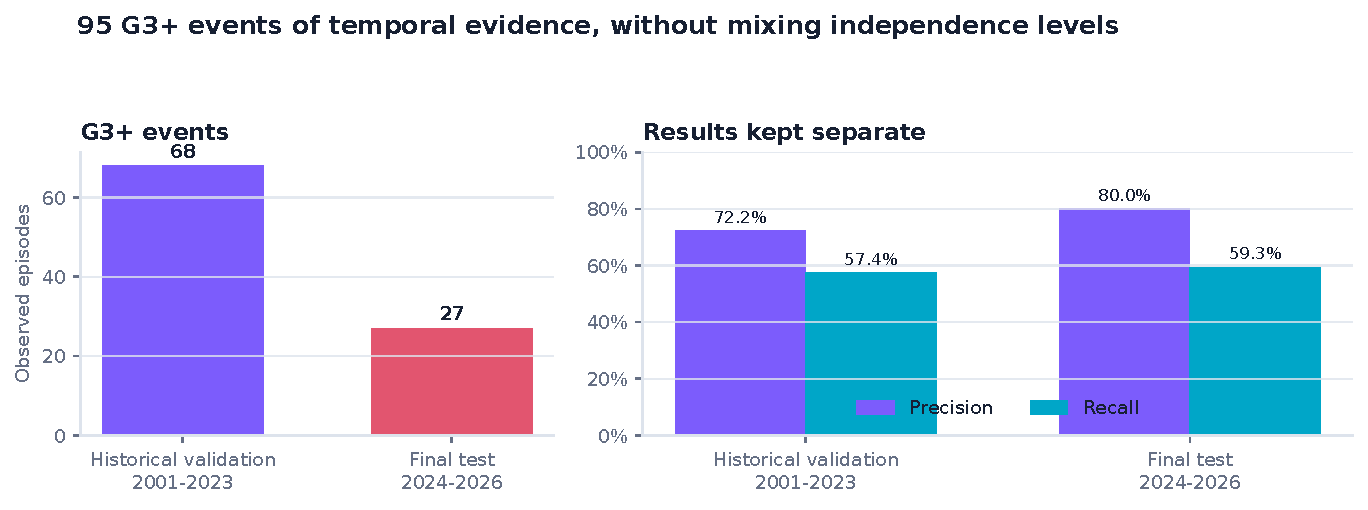
\includegraphics[width=0.92\textwidth]{figures-en/evidence-split.pdf}
\caption{Historical validation adds context while the final test preserves independence. The two scores are not merged into a single figure.}
\end{figure}

\section{Four similar-looking products that are not equivalent}

NOAA forecast, HelioSat, and GFZ nowcast all publish numbers that look like Kp, but they answer different questions. Comparing them without showing their lead time would produce the wrong conclusion.

\newpage
\begin{table}[H]
\centering
\small
\begin{tabularx}{\textwidth}{>{\bfseries}p{30mm}p{24mm}p{31mm}X}
\toprule
Product & Type & Lead time & Correct interpretation\\
\midrule
NOAA next day & Forecast & 23.5 - 44.5 h & Long lead time; it has not yet observed at L1 the structure that will arrive the next day.\\
NOAA two day & Forecast & 47.5 - 68.5 h & A still harder horizon; it provides strategic context, not a last-minute alarm.\\
HelioSat & Forecast & Median 47 min & It has already observed the parcel at L1 and estimates its arrival and impact. Less horizon, but more direct physical information.\\
GFZ nowcast & Nowcast & No positive lead & It estimates the geomagnetic response that is already happening or has just happened. It is a reference, not a predictive competitor.\\
GFZ definitive & Final observation & Retrospective & This is the truth used to score all other products.\\
\bottomrule
\end{tabularx}
\end{table}

To make the comparison fair, we use exactly the same \textbf{3,694 intervals}, from 3 January 2025 to 30 April 2026. Only one daily NOAA issue is retained, the 00:30 UTC issue. This common subset contains 90 G1+ episodes and 14 G3+ episodes.

\begin{figure}[H]
\centering
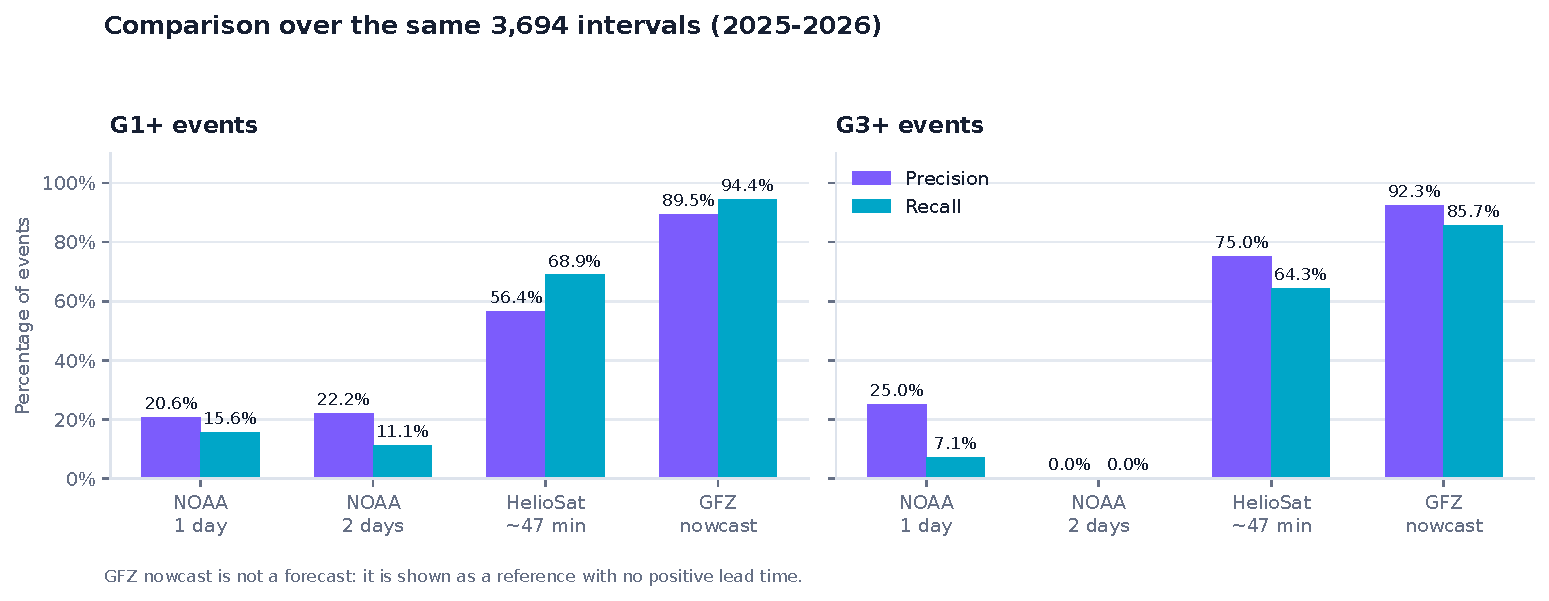
\includegraphics[width=\textwidth]{figures-en/product-comparison.pdf}
\caption{Event-level precision and recall. The strong GFZ nowcast result must be interpreted alongside its lack of positive lead time. The G3+ comparison contains only 14 events and therefore carries high uncertainty.}
\end{figure}

The practical interpretation is:
\begin{itemize}
  \item \textbf{NOAA provides time to prepare}, but recall is low in this archive when we require it to identify the exact Kp episode.
  \item \textbf{HelioSat provides less time}, around 47 minutes in the common subset, but detects a much larger fraction of episodes because it has already measured the solar structure at L1.
  \item \textbf{GFZ nowcast is the closest to the definitive value}, as expected: it describes a terrestrial response already under way rather than anticipating it.
\end{itemize}

\begin{warningbox}
This figure does not show that HelioSat is generally "better than NOAA." It shows that the systems solve different tasks: NOAA looks one or two days ahead, while HelioSat issues a short-term physical alert after the disturbance has reached L1.
\end{warningbox}

\section{Hits, false alarms, and missed storms}

For clarity, consecutive Kp intervals are grouped into episodes. A nine-hour storm does not count as three independent cases. An alert and a storm are matched if they overlap within a predefined tolerance of one Kp bin, or three hours.

\begin{table}[H]
\centering
\begin{tabularx}{\textwidth}{>{\bfseries\raggedright\arraybackslash}p{32mm}>{\raggedright\arraybackslash}p{48mm}>{\raggedright\arraybackslash}X}
\toprule
Concept & What happened & Plain-language meaning\\
\midrule
True positive (TP) & We alerted and a storm occurred & A hit\\
False positive (FP) & We alerted and no matching storm occurred & A false alarm\\
False negative (FN) & We did not alert and a storm did occur & A missed storm\\
True negative (TN) & We did not alert and no storm occurred & A quiet period correctly ignored\\
\bottomrule
\end{tabularx}
\end{table}

\textbf{Precision} asks: "when we issued an alert, how often were we right?" It is calculated as $TP/(TP+FP)$. \textbf{Recall} asks: "of all the real storms, how many did we find?" It is calculated as $TP/(TP+FN)$.

\begin{figure}[H]
\centering
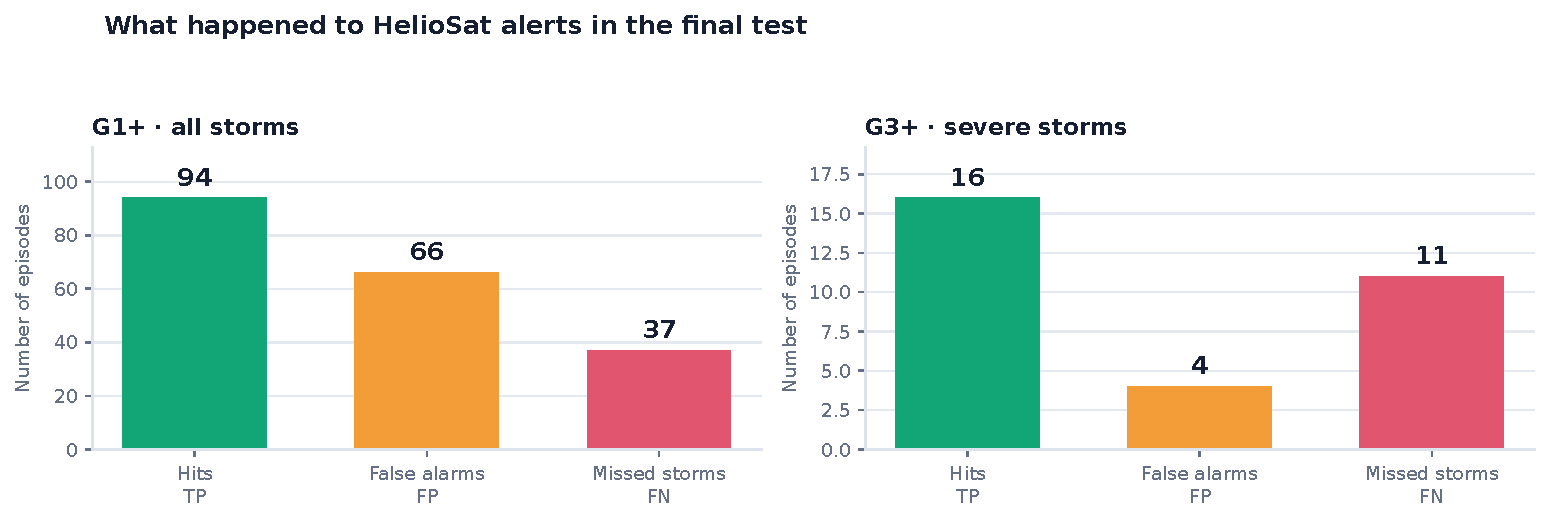
\includegraphics[width=\textwidth]{figures-en/event-outcomes.pdf}
\caption{Results of the HelioSat candidate on the final test from 2024 to April 2026.}
\end{figure}

\begin{table}[H]
\centering
\small
\caption*{Episode-level summary}
\begin{tabular}{lrrrrrr}
\toprule
Threshold & Real events & TP & FP & FN & Precision & Recall\\
\midrule
G1+ / Kp $\geq 5$ & 131 & 94 & 66 & 37 & 58.8\% & 71.8\%\\
G3+ / Kp $\geq 7$ & 27 & 16 & 4 & 11 & 80.0\% & 59.3\%\\
\bottomrule
\end{tabular}
\end{table}

For G3+, eight out of ten alerts were correct, but the system found approximately six out of ten real storms. Precision is good; the main room for improvement is reducing the eleven missed severe storms. The operational threshold should be selected according to the actual cost of a false alarm versus the cost of failing to warn of a G3+ storm.

\section{What changed when the model was properly trained}

The previous version was a fixed physical rule based mainly on speed and southward magnetic field. It was interpretable, but it did not learn from historical cases. The new candidate combines 59 features, fits G1+ and G3+ probabilities separately, and also produces a continuous Kp estimate.

\newpage
\begin{figure}[H]
\centering
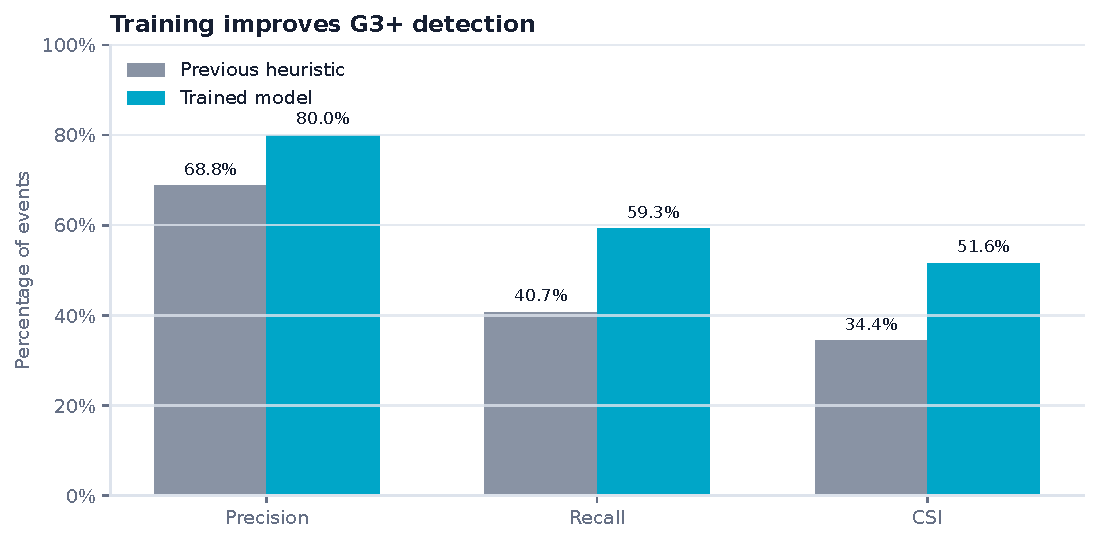
\includegraphics[width=0.76\textwidth]{figures-en/baseline-improvement.pdf}
\caption{G3+ comparison on the same final test. CSI combines hits, false alarms, and missed events in a single metric.}
\end{figure}

\begin{center}
\begin{tabular}{lrr}
\toprule
Continuous metric & Previous heuristic & Trained model\\
\midrule
Mean absolute Kp error & 0.92 & \textbf{0.44}\\
Kp RMSE & 1.13 & \textbf{0.57}\\
Correlation with definitive Kp & 0.754 & \textbf{0.918}\\
Mean Kp bias & +0.63 & \textbf{+0.05}\\
\bottomrule
\end{tabular}
\end{center}

The improvement is not limited to estimating a closer Kp value. For G3+, the model increases the number of detected storms from 11 to 16 and reduces false alarms from five to four. Recall rises from 40.7\% to 59.3\%, while precision increases from 68.8\% to 80.0\%.

\section{An example: the May 2024 storm}

The May 2024 storm is a useful example because it belongs entirely to the final test. The model did not use this episode during training or to select its thresholds.

\begin{figure}[H]
\centering
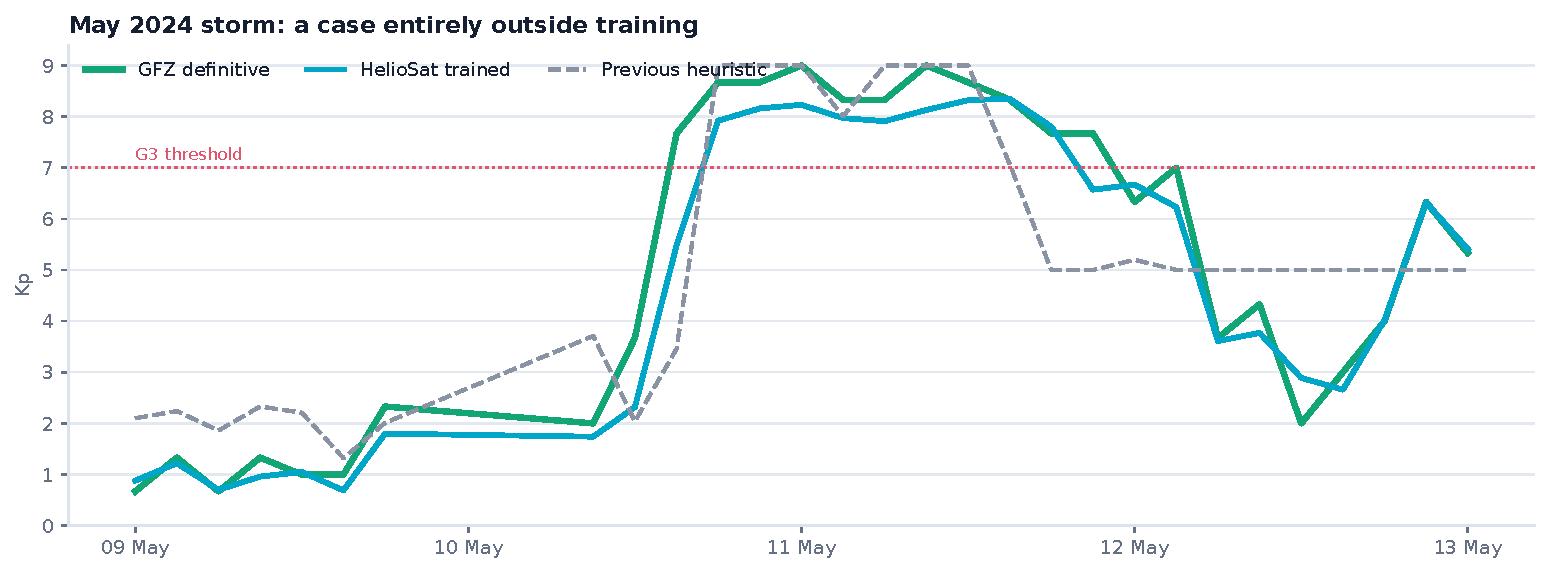
\includegraphics[width=\textwidth]{figures-en/may-2024-episode.pdf}
\caption{Evolution of definitive Kp, the candidate estimate, and the previous heuristic. Each point still represents an official three-hour Kp interval.}
\end{figure}

The candidate follows the main rise closely and reproduces the severe phase much better than the previous rule. Even so, the chart also shows why the full validation should not be reduced to one spectacular case: commercial performance is determined by all 27 G3+ storms in the test, including the eleven it missed.

\section{What we can claim and what remains to be done}

\begin{summarybox}
\textbf{A reasonable claim today.} The trained candidate materially improves on the previous heuristic and produces a useful short-term signal for severe storms. In the final test, it achieved 80.0\% G3+ precision and 59.3\% G3+ recall, with a median L1-to-Earth transit time of 51 minutes.
\end{summarybox}

\textbf{We should not yet claim} that live precision will be exactly the same, that a 51-minute SLA exists, or that HelioSat replaces NOAA's one- or two-day forecast. There are three reasons:
\begin{itemize}
  \item The test contains only 27 G3+ episodes; the recall confidence interval is 40.7\% - 75.5\%.
  \item OMNI applies retrospective phase-front processing. Live operations will have different latency and data quality.
  \item Kp aggregates three hours and cannot measure response onset with minute-level accuracy.
\end{itemize}

\subsection{Next steps}

\begin{enumerate}
  \item \textbf{Shadow mode.} Run the candidate without driving customer alerts yet, and store every issue with its issue time, version, and available features.
  \item \textbf{Immutable live validation.} Compare those issues with GFZ definitive without retrospectively changing the model or threshold.
  \item \textbf{Two temporal targets.} Keep Kp/G3 for NOAA compatibility and add GFZ Hp30 as a 30-minute label for studying onset, duration, and peaks. GFZ presents Hp30 specifically as a temporal improvement over Kp.\source{3}
  \item \textbf{Cost-based threshold.} Select how many false alarms to accept in exchange for fewer missed G3+ storms, according to each customer's use case.
  \item \textbf{Update the external comparison.} Continue archiving NOAA issues and GFZ nowcasts over the same bins to avoid biased comparisons.
\end{enumerate}

\section{Sources and traceability}

\small
\begin{enumerate}
  \item NASA Space Physics Data Facility. \textit{High Resolution OMNI: one-minute and five-minute solar-wind data sets at the Earth's bow shock nose}. \url{https://omniweb.gsfc.nasa.gov/html/HROdocum.html}
  \item GFZ Helmholtz Centre for Geosciences. \textit{About Kp index} and the definitive/nowcast Kp data service. \url{https://kp.gfz.de/en/about-kp} and \url{https://kp.gfz.de/en/data}
  \item GFZ Helmholtz Centre for Geosciences. \textit{About Hpo: Hp30 and Hp60}. \url{https://kp.gfz.de/en/hp30-hp60/about-hpo}
  \item NOAA SWPC / NCEI. \textit{Issued three-day planetary Kp forecast archive}. \url{https://www.ngdc.noaa.gov/stp/space-weather/swpc-products/daily_reports/3day_forecast/}
  \item Newell, P. T. et al. (2007). \textit{A nearly universal solar wind-magnetosphere coupling function inferred from 10 magnetospheric state variables}. Journal of Geophysical Research. \url{https://doi.org/10.1029/2006JA012015}
\end{enumerate}

\vfill
\begin{resultbox}
\scriptsize\color{Muted}\textbf{Reproducible artefacts.} This report was generated from \texttt{geomagnetic-storm-study.json} and model \texttt{gbdt-coupling-probability-v2}. Hyperparameters and thresholds were selected using four chronological validation blocks ending in 2023. All headline metrics come from January 2024 to April 2026. The NOAA/GFZ comparison uses only the 3,694 common bins available from January 2025.
\end{resultbox}

\end{document}
